\documentclass{beamer}
\usetheme{Padova}
\usepackage{presentazione}

\title{\textsc{Classificazione di attività motorie tramite accelerometro del cellulare}}
\author{Galtarossa Luisa\and Grassi Alberto\and Montin Anna\and Zago Daniele}
\date{}

\begin{document}
\begin{frame}
\titlepage
\end{frame}

\section{Introduzione}
\begin{frame}{Il problema analizzato}
Ormai con il cellulare è possibile fare moltissime cose. 
Cancellare messaggi, avere più giga...è tutto possibile con un solo shake.\\
\smallskip
Ma come possiamo riconoscere uno shake?
\begin{figure}[H]

\includegraphics[width=0.4\textwidth]{./images/vodafoneshake.png}
\end{figure}
\end{frame}

\begin{frame}{La nostra idea}
Riconoscere uno shake tra diverse attività motorie.\\
\smallskip
\begin{columns}[T] % align columns
\begin{column}{.48\textwidth}
Le attività analizzate sono:
\begin{itemize}
\item Camminata
\item Camminata con cellulare in tasca
\item Corsa
\item Corsa con cellulare in tasca
\item Utilizzo a riposo
\item Salti
\item Salita e discesa di scale
\end{itemize}
\end{column}%
\hfill%
\begin{column}{.4\textwidth}
\begin{figure}[H]
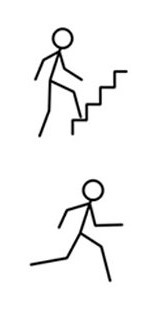
\includegraphics[width=0.6\textwidth]{./images/attivit.jpg}
\end{figure}
\end{column}%
\end{columns}
\end{frame}

\begin{frame}{Raccolta dati}
I dati sono stati raccolti tramite l'applicazione \cite{kumarPhonePiSampleServer2019}.\\
\smallskip
Questa fornisce l'accelerazione in forma vettoriale ad ogni istante $t$.
\[
\vec{a_t} = \begin{pmatrix}
a_x \\ a_y \\ a_z
\end{pmatrix}
\]
\end{frame}

\begin{frame}{Accelerazione}
L'accelerazione viene calcolata come $\|\vec{a_t}\| =\sqrt{a_x^2+a_y^2+a_z^2}$.
\begin{table}[H]
\begin{tabular}{cccccccc}
\toprule
y & $\|\vec{a}_0\|$ & $\|\vec{a}_1\|$ & $\|\vec{a}_2\|$  & $\dots$ & $\|\vec{a}_{149}\|$\\
\midrule
camminata & 5.449 & 5.300 & 5.344 &  $\cdots$ & 13.147\\
camminata & 13.977 & 14.910 & 15.567 &  $\cdots$ & 5.480\\
camminata & 5.608 & 5.868 & 6.143 &  $\cdots$ & 18.227\\
camminata & 19.026 & 18.886 & 18.098 &  $\cdots$ & 6.299\\
$\vdots$ & $\vdots$ & $\vdots$ & $\vdots$ &  $\cdots$ & $\vdots$\\
shake & 11.480 & 14.663 & 16.968 &  $\cdots$ & 8.474\\

\bottomrule
\end{tabular}
\end{table}
Perché non lavorare direttamente con le esplicative $a_0,\dots,a_{149}$?
\end{frame}

\section{Esplorative}
\begin{frame}
\begin{figure}[H]
\includegraphics[width=\textwidth]{../figure/espl.png}
\end{figure}
\end{frame}


\begin{frame}

\begin{columns}[T] % align columns
\begin{column}{.48\textwidth}
\begin{figure}[H]
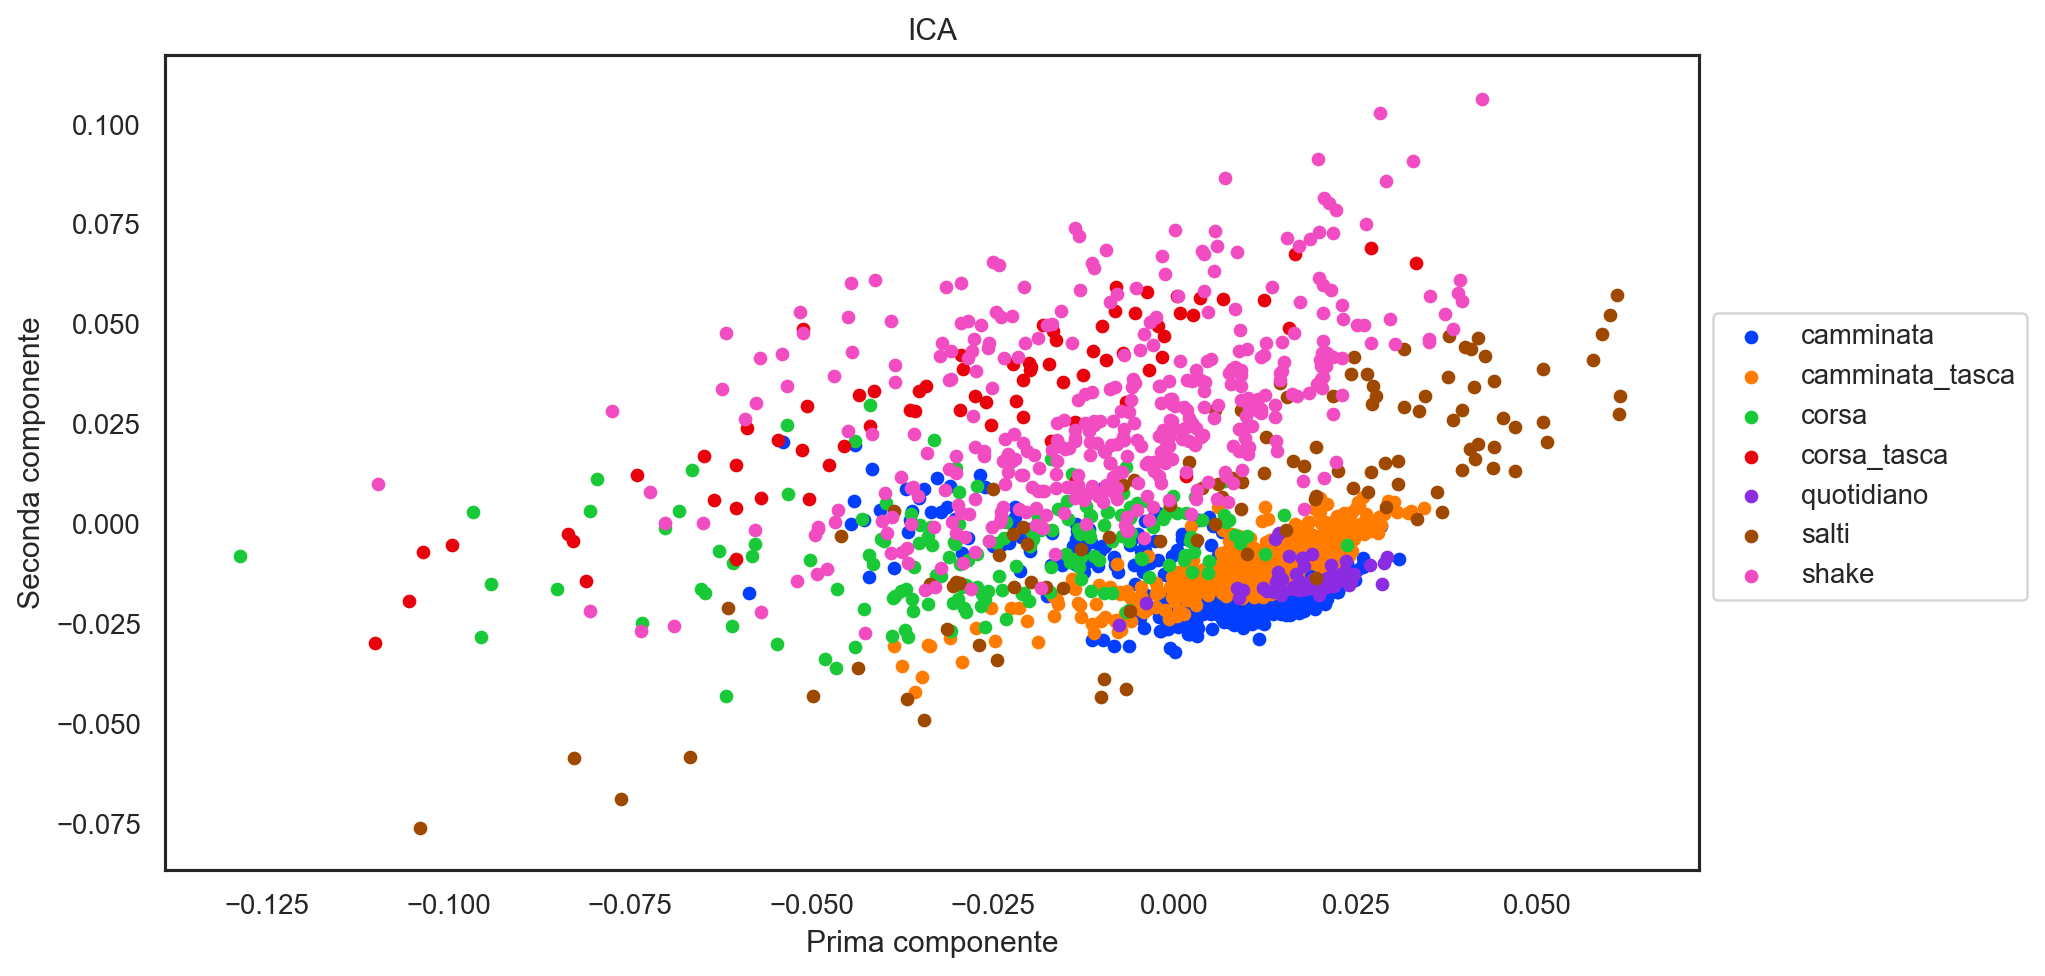
\includegraphics[width=\textwidth]{../figure/ICA.png}
\end{figure}
\end{column}%
\hfill%
\begin{column}{.48\textwidth}
$f(x)=x^2$
\end{column}%
\end{columns}
\end{frame}
%\documentclass[./main.tex]{subfiles}

\begin{document}
\section{Analisi esplorativa}
Per condurre una prima analisi esplorativa si sono considerati i grafici dell'accelerazione rispetto al tempo (ms) per le diverse attività registrate; da ogni misurazione sono stati tolti i primi e gli ultimi sette secondi ottenendo le seguenti rappresentazioni:
\begin{figure}[H]
	\centering
	\includegraphics[width=.8\textwidth, keepaspectratio]{../../figure/espl.png}
	\caption{{}}
	\label{espl}
\end{figure}
In generale, per le varie attività registrate si osserva che l'intensità dell'accelerazione e la frequenza dei picchi sono entrambe piuttosto basse per "camminata", "camminata tasca", "corsa" e "quotidiano". La differenza inizia ad emergere nello studio di "salti", "corsa tasca" e "shake".
\\
Emerge chiaramente come il segnale sia molto differente per queste tre diverse attività. In particolare si nota
una differenza nell'intensità (più bassa per lo shake e maggiore negli altri due casi) e nella frequenza (la quale cresce passando da "cosa tasca" a "salti" fino a "shake"). Anche i picchi che vengono raggiunti sono diversi nei vari casi: nel primo si hanno picchi fino a $90\si{\metre\per\square\second}$ ma poco frequenti; nel secondo si notano picchi di intensità lievemente inferiore ma molto più ravvicinati. Infine lo shake evidenzia un segnale molto denso con  picchi piuttosto bassi rispetto ai precedenti. 
\\

Successivamente sono stati sbiancati i dati e sono state applicate le seguenti tecniche d'analisi:
\begin{itemize}
	\item PCA sui dati sbiancati.
	\item ICA sui dati sbiancati.
	\item t-SNE sui dati sbiancati.
\end{itemize}
Le prime due componenti principali non riescono a isolare adeguatamente i vari segnali; l'analisi delle componenti indipendenti non migliore il risultato dal momento che quest'ultima rappresenta una rotazione della prima. Un output migliore lo si ottiene mediante il t-SNE (figura \ref{t-sne}). 
\begin{figure}[H]
	\centering
	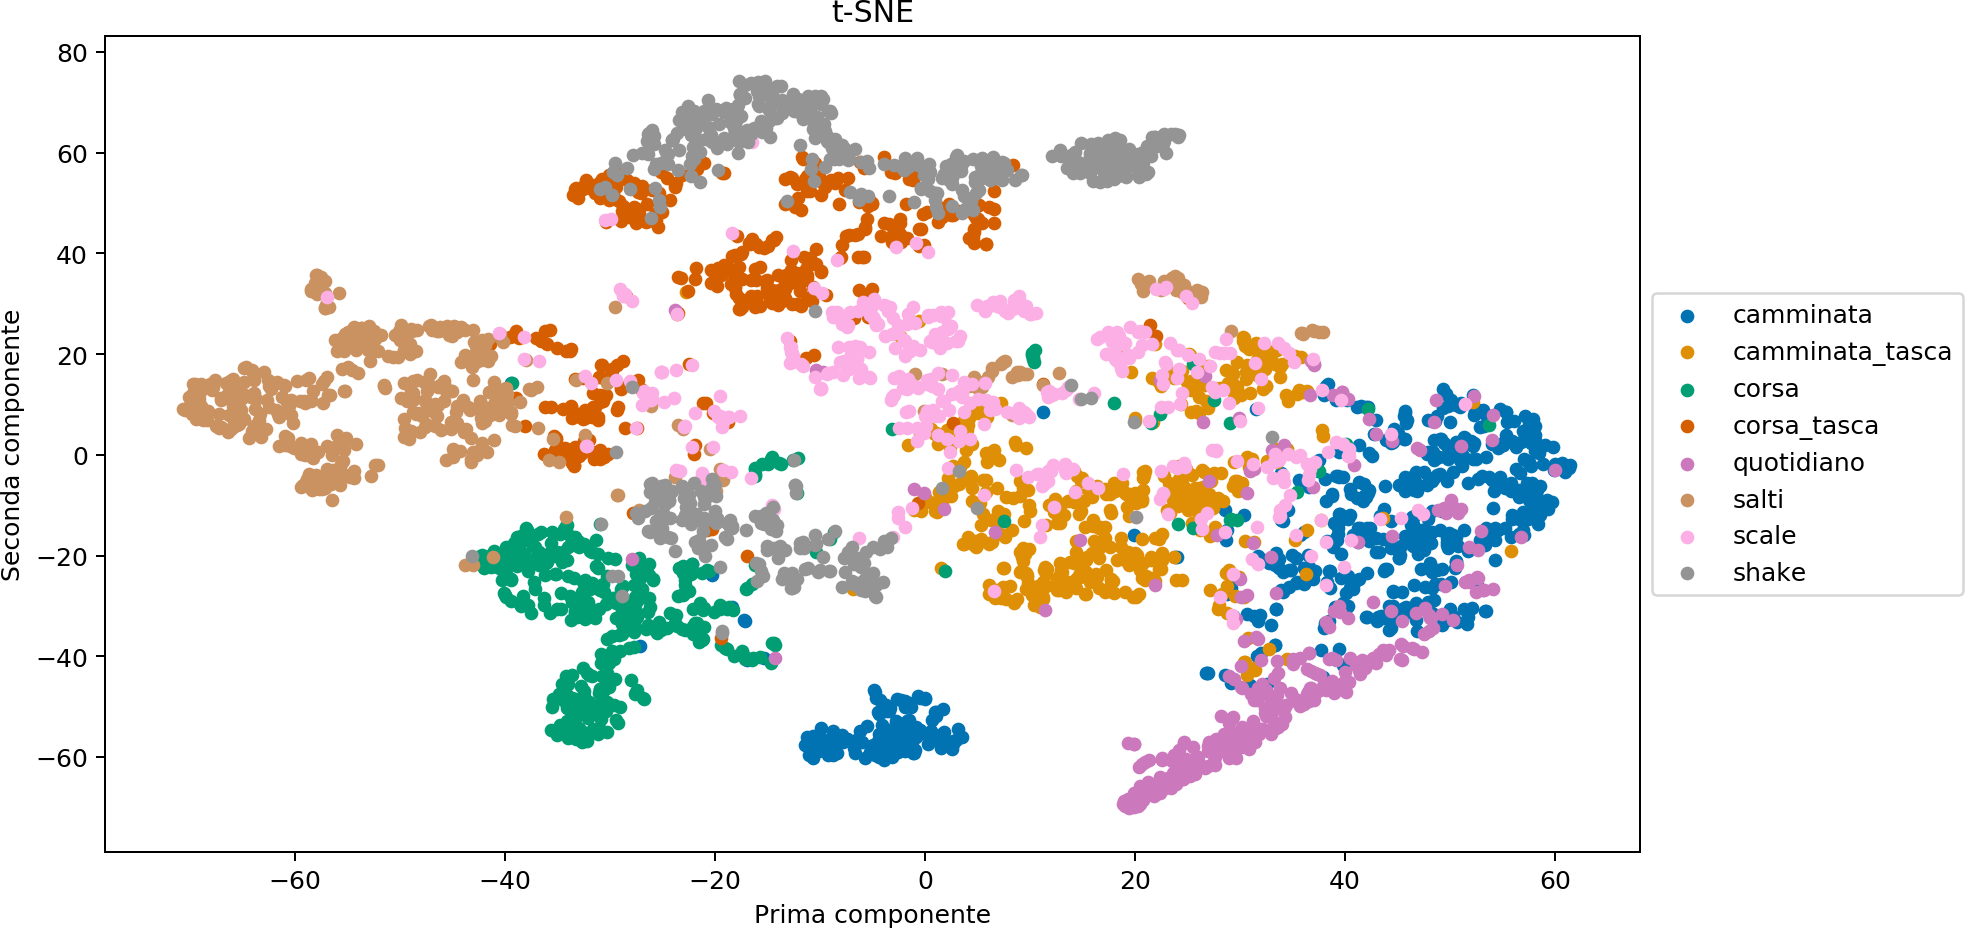
\includegraphics[width=.8\textwidth, keepaspectratio]{../../figure/t-SNE.png}
	\caption{{ t-SNE per i dati sbiancati}}
	\label{t-sne}
\end{figure}
Si osserva in particolare come l'attività di interesse, ovvero lo shake, venga principalmente confusa con "corsa" e "corsa tasca". 
\\
Tale problema rappresenta il punto di partenza per un'analisi volta a classificare correttamente i vari segnali nelle diverse categorie.

\textcolor{red}{EVENTUALE COMMENTO SULLE DISTRIBUZIONI DELLE ESPLICATIVE SCELTE}

\section{Appendice}
\begin{figure}[H]
	\centering
	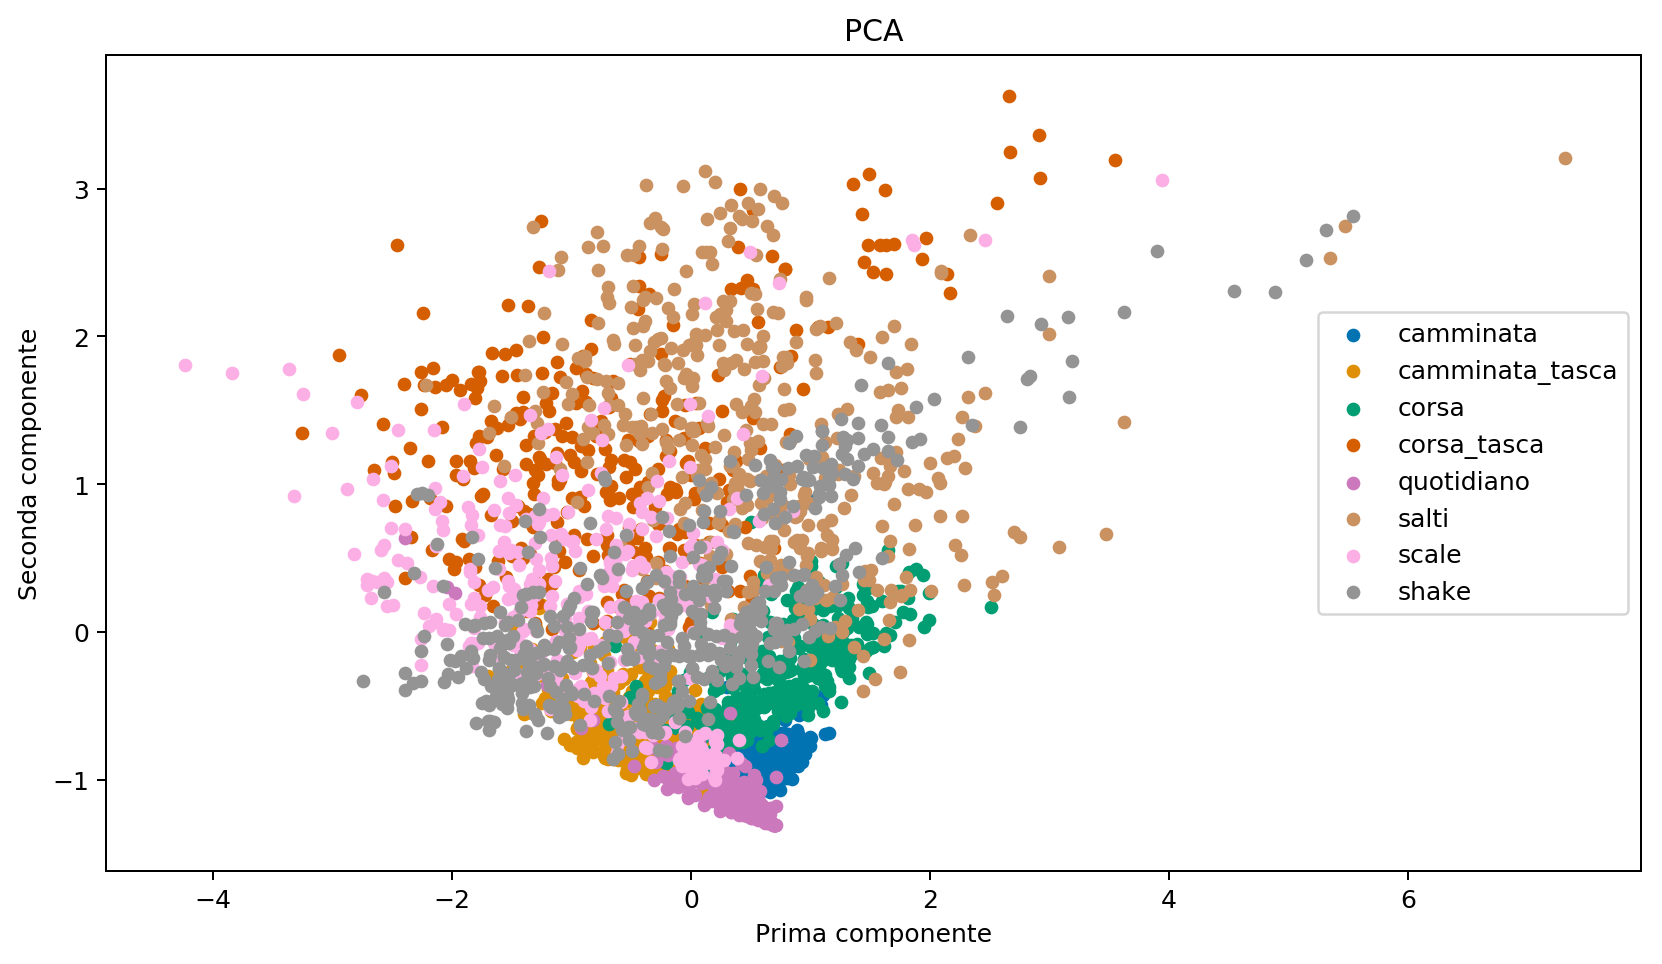
\includegraphics[width=.8\textwidth, keepaspectratio]{../../figure/PCA.png}
	\caption{{ Prime due componenti principali per i dati sbiancati}}
	\label{PCA}
\end{figure}
\end{document}
%\input{tex/...}

%\printbibliography

\end{document}